\chapter{Premier Classeur}
\section{Création d’un nouveau classeur}
 \begin{center} 
	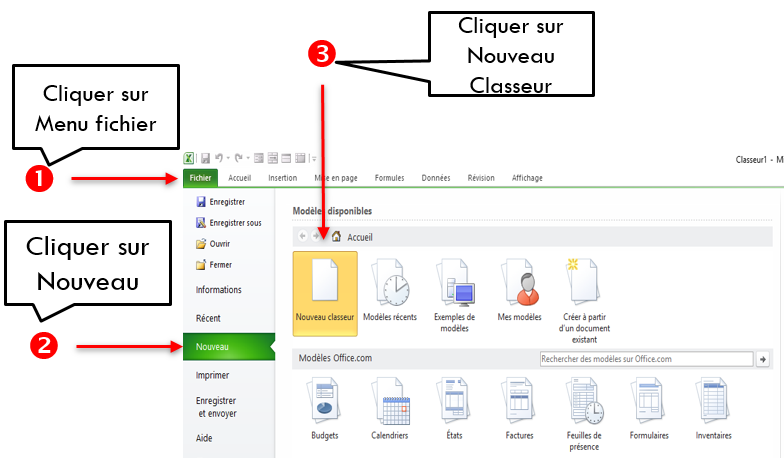
\includegraphics[scale=0.2,width=\linewidth]{img/nouveau_classeur} 
	\captionof{figure}{Création d’un nouveau classeur}
\end{center}
 \begin{center} 
	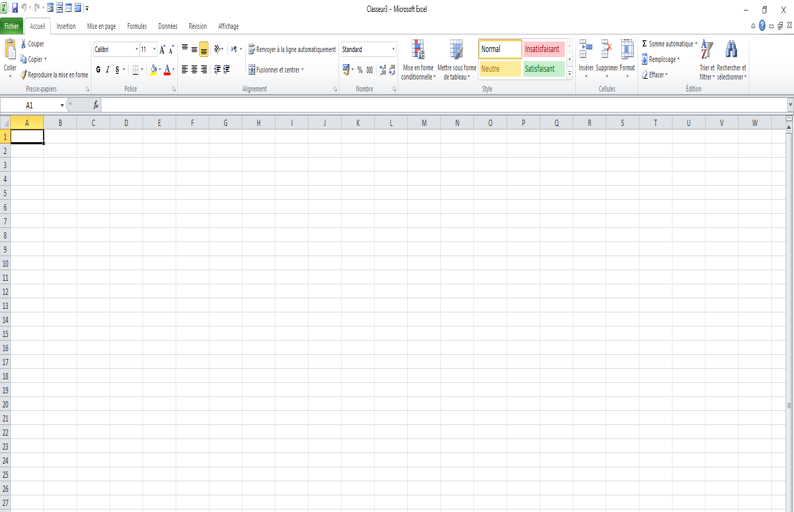
\includegraphics[scale=0.2,width=\linewidth]{img/classeur} 
	\captionof{figure}{Nouveau Classeur}
\end{center}
\section{Enregistrer un classeur la première fois}
\begin{center} 
	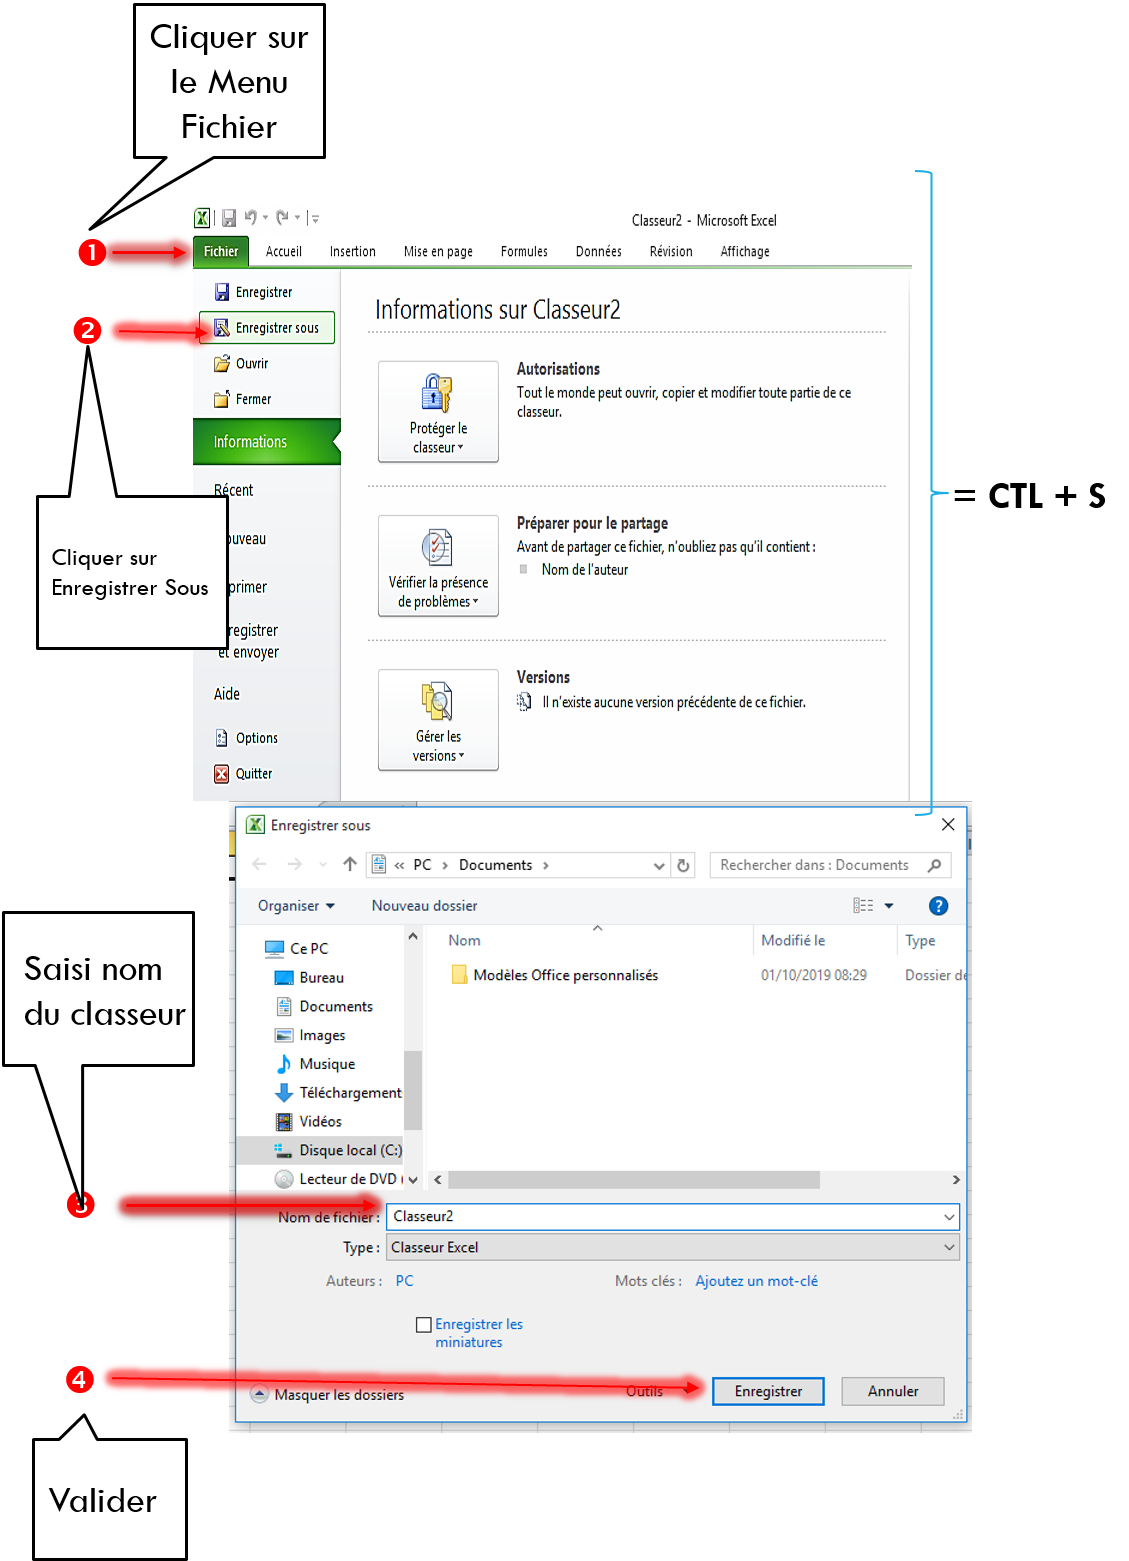
\includegraphics[scale=0.2,width=\linewidth]{img/sauve_as_classeur} 
	\captionof{figure}{Enregistrement d'un classeur la premiere fois} 
\end{center}

\section{Enregistrer les autres fois}
\begin{center} 
	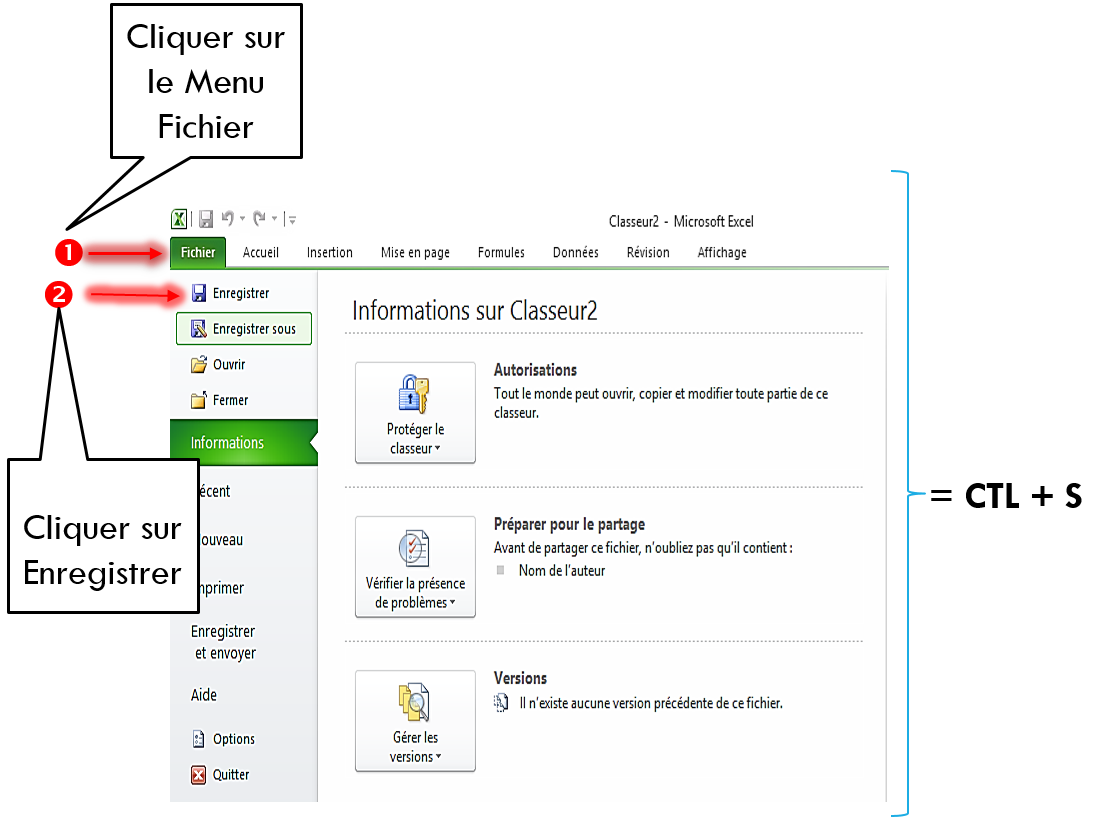
\includegraphics[scale=0.2,width=0.8\linewidth]{img/sauve_classeur} 
	\captionof{figure}{Enregistrement d'un classeur} 
\end{center}
\section{Fermeture d'un classeur}
\begin{center} 
	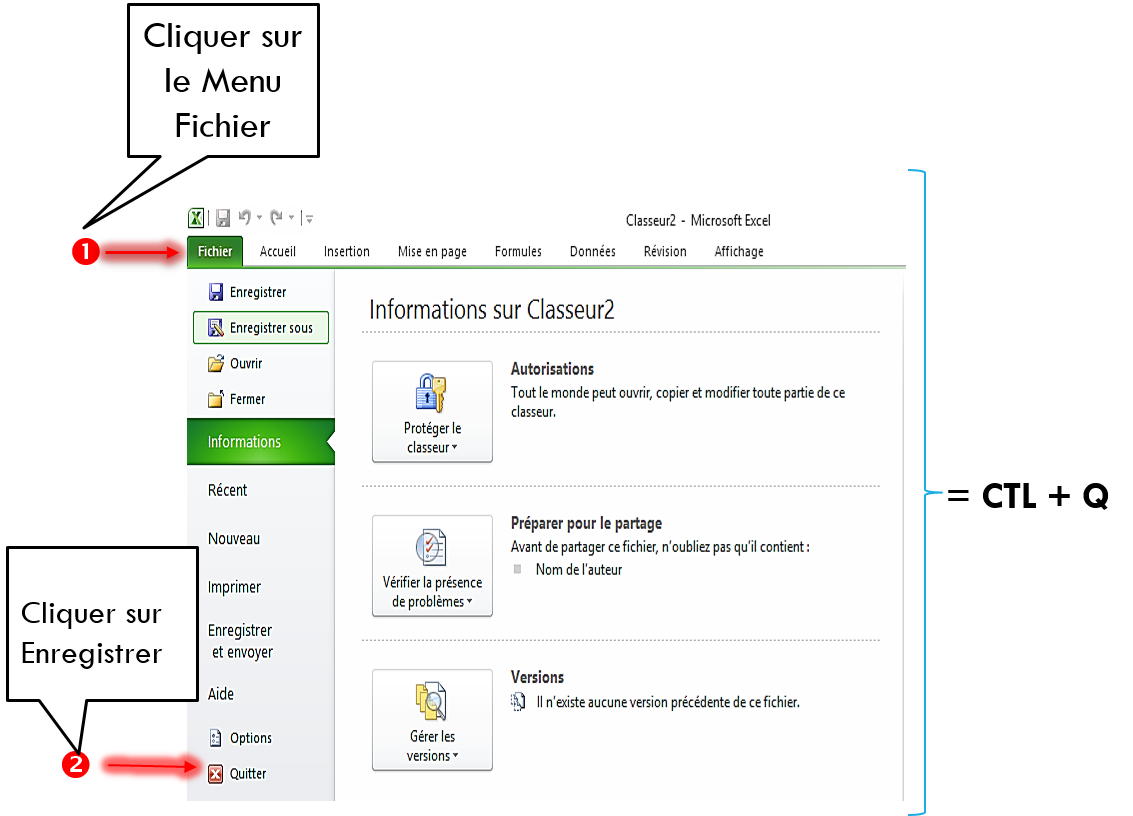
\includegraphics[scale=0.2,width=0.8\linewidth]{img/close_classeur} 
	\captionof{figure}{Fermeture d'un classeur} 
\end{center}

\section{ Saisir du texte et des nombres }
\subsection{ Saisir du texte}
\begin{center} 
	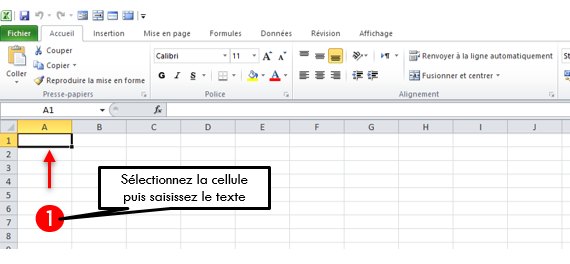
\includegraphics[scale=0.2,width=0.6\linewidth]{img/selecte_cellule} 
 
\end{center}
\begin{center} 
	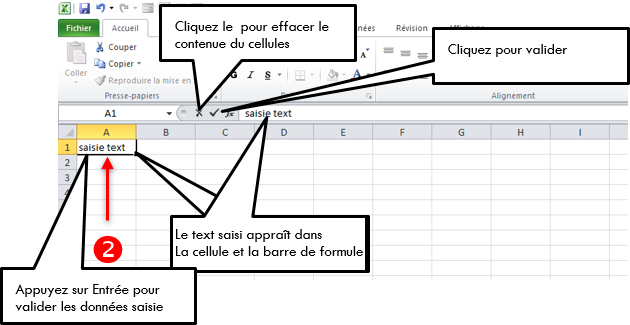
\includegraphics[scale=0.2,width=0.7\linewidth]{img/saisie_text} 
	\captionof{figure}{Saisie du Text} 
\end{center}
\subsection{ Saisir des nombres }
\begin{center} 
	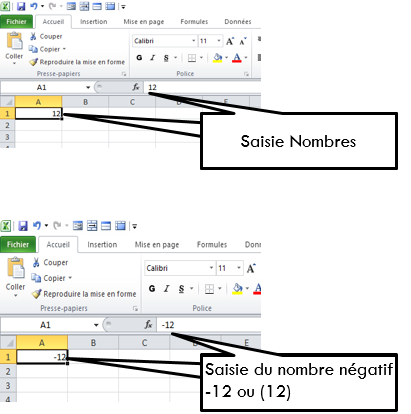
\includegraphics[scale=0.2,width=0.6\linewidth]{img/saisie_nombre} 
	\captionof{figure}{Saisie des nombres} 
\end{center}
\section{Modifier des données} 
\begin{center} 
	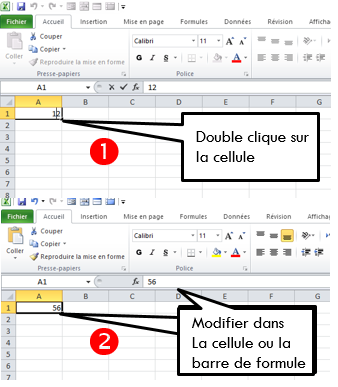
\includegraphics[scale=0.2,width=0.6\linewidth]{img/modification_donner} 
	\captionof{figure}{Modication de donnée} 
\end{center}
\section{Supprimer les données} 
\begin{center} 
	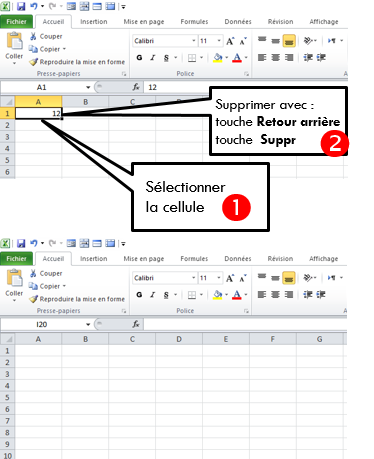
\includegraphics[scale=0.2,width=0.5\linewidth]{img/delete_donner} 
	\captionof{figure}{Supprimer les données} 
\end{center}
\section{Déplacez ou copiez des données} 
	\begin{center} 
		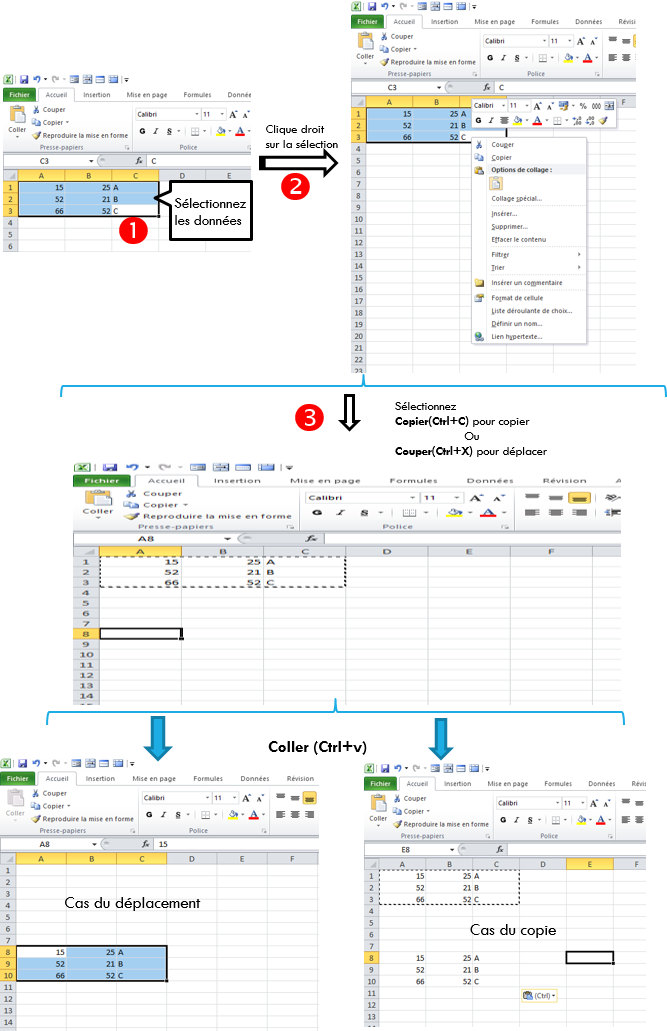
\includegraphics[scale=0.2,width=0.9 \linewidth]{img/deplacer_donner} 
		\captionof{figure}{Supprimer les données} 
	\end{center}
\section{Agrandir les cellules} 
\begin{center} 
	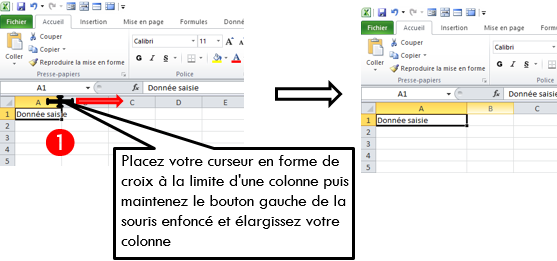
\includegraphics[scale=0.2,width=0.9 \linewidth]{img/agrandir_cellule} 
	\captionof{figure}{Agrandire Cellule} 
\end{center}
\section{Formats,  mise en forme et poignée de recopie incrémentée}
\subsection{Formats}
\begin{center} 
	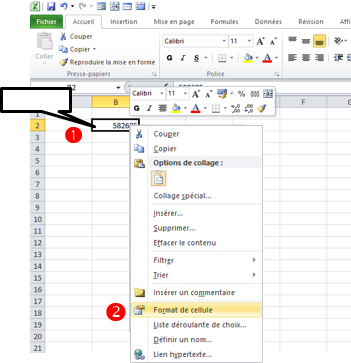
\includegraphics[scale=0.2,width=0.7 \linewidth]{img/format1} 
\end{center}
 \begin{center}  
 	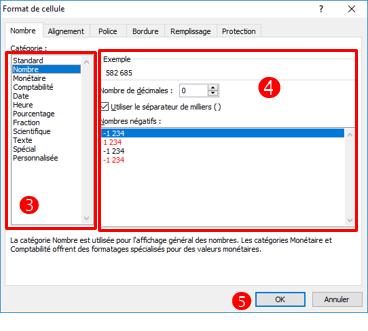
\includegraphics[scale=0.2,width=0.7 \linewidth]{img/format2}
 	\captionof{figure}{Format de donnée} 
 \end{center}
\begin{Exemple}
Cette exemple illustre l'utilisation de formats des nombres
\end{Exemple} 
\begin{center}  
	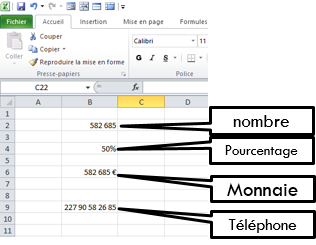
\includegraphics[scale=0.2,width=0.7 \linewidth]{img/exemple_format}
	\captionof{figure}{Exemple Format des nombres} 
\end{center}

\subsection{Mise en forme}
\subsubsection{Bordure}
\begin{center}  
	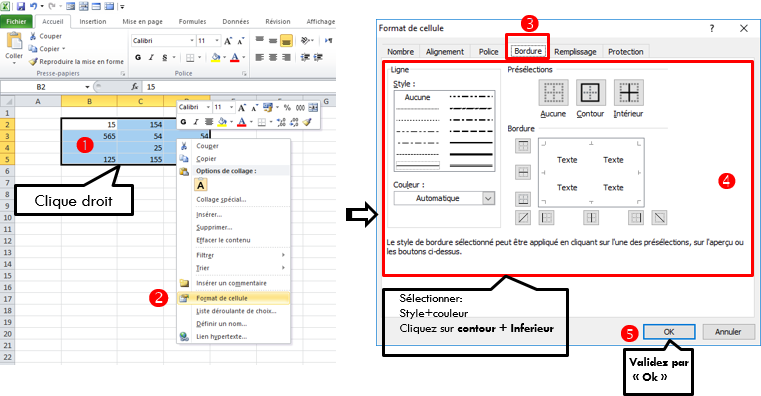
\includegraphics[scale=0.2,width=0.9 \linewidth]{img/bordure_cellule}
		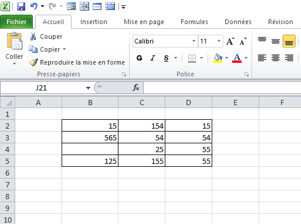
\includegraphics[scale=0.2,width=0.9 \linewidth]{img/tableau_bordure}
	\captionof{figure}{Bordure des cellules} 
\end{center}
\subsubsection{Aligments}
\begin{center}  
	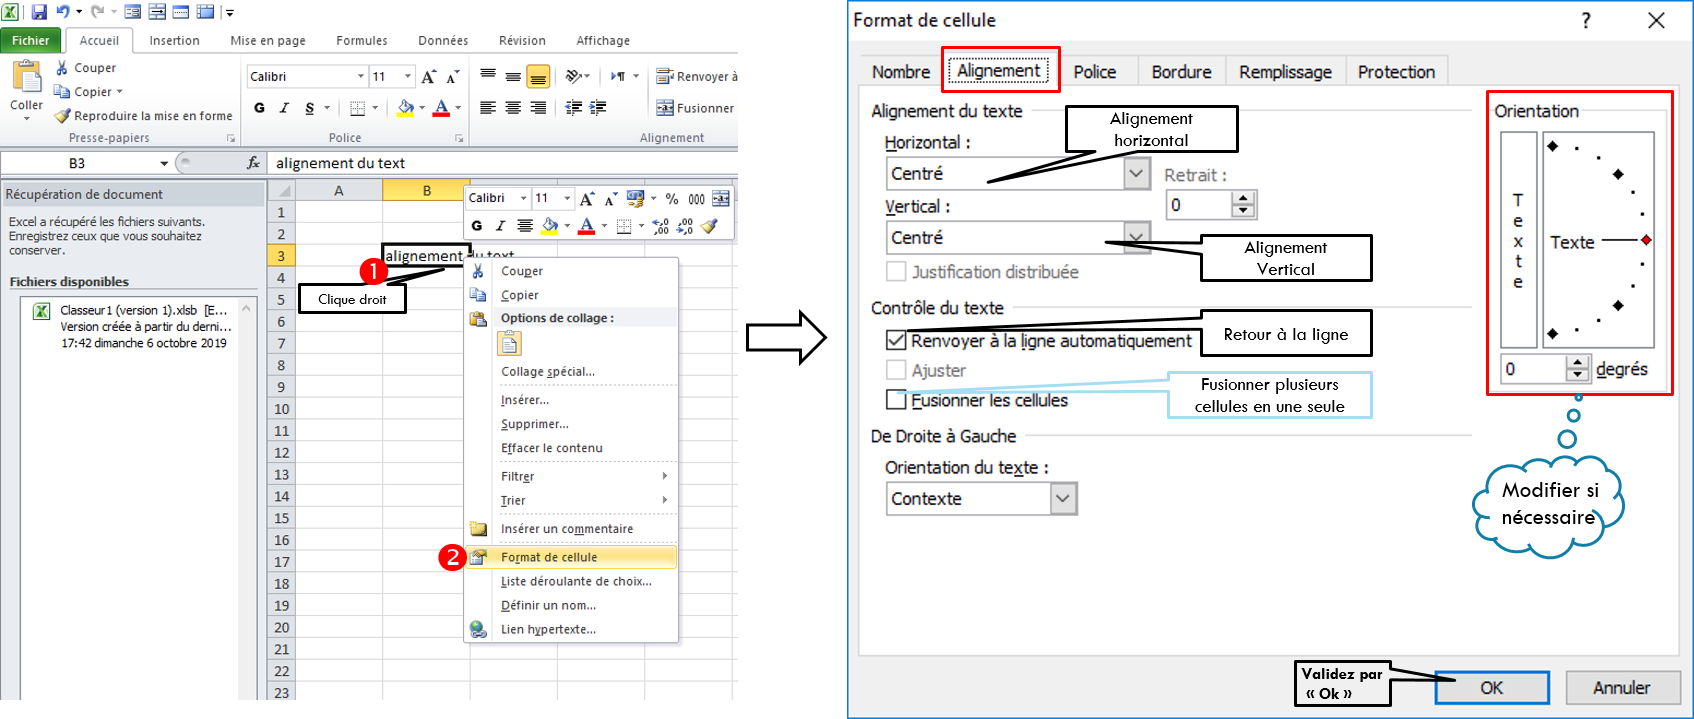
\includegraphics[scale=0.2,width= \linewidth]{img/aligment_text}
	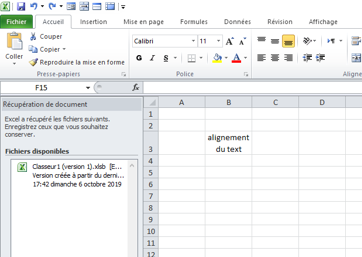
\includegraphics[scale=0.2,width= \linewidth]{img/aligment_exemple}
	\captionof{figure}{Aligment text} 
\end{center}
\subsubsection{Police}
\begin{center}  
	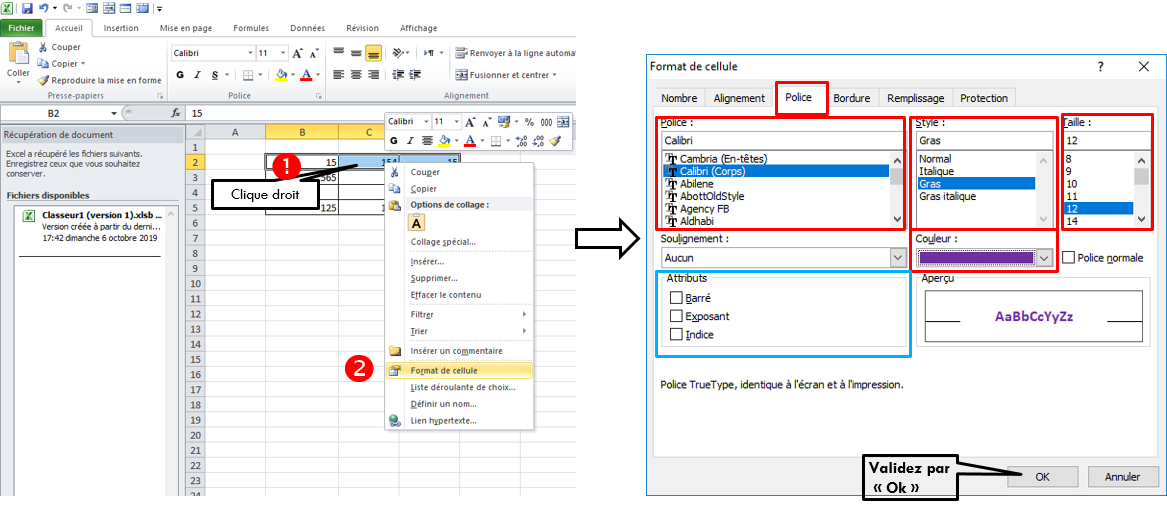
\includegraphics[scale=0.2,width= \linewidth]{img/police_text}
	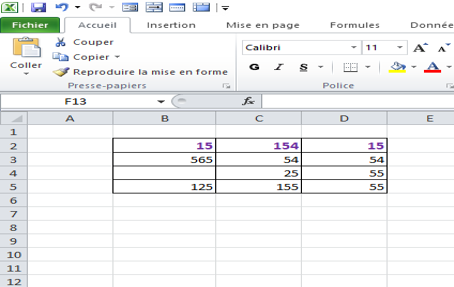
\includegraphics[scale=0.2,width= \linewidth]{img/police_exemple}
	\captionof{figure}{Police text} 
\end{center}
\subsubsection{Trames des Cellules}
\begin{center}  
	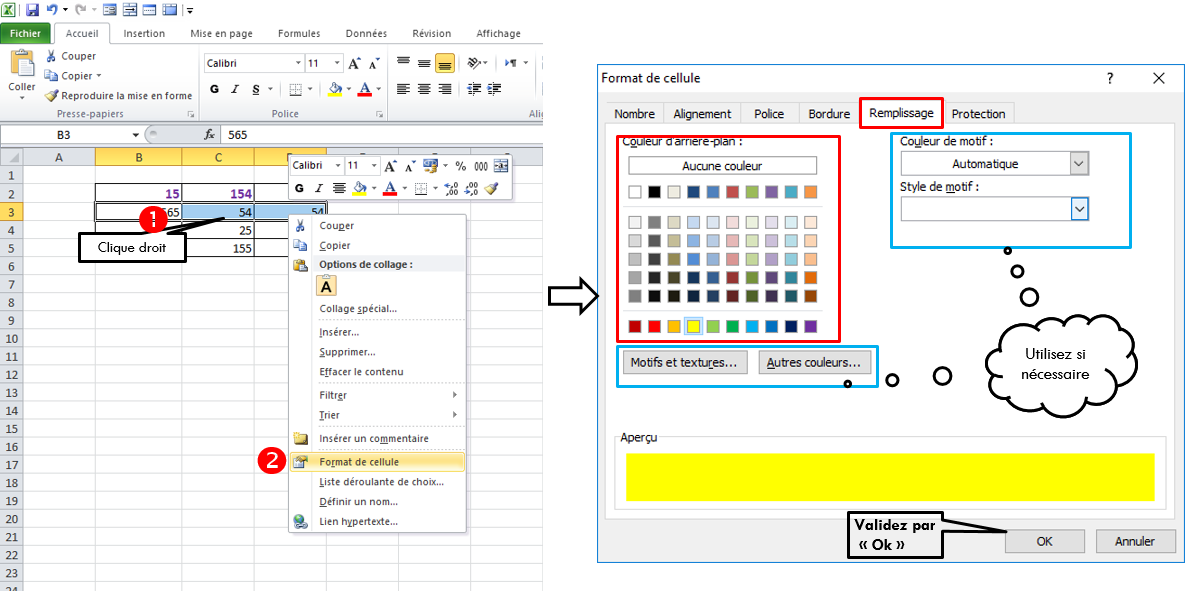
\includegraphics[scale=0.2,width= \linewidth]{img/trame_cellule}
	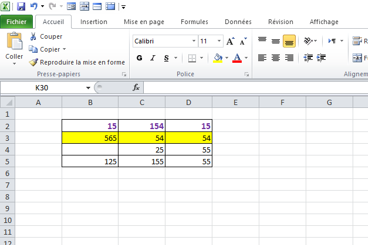
\includegraphics[scale=0.2,width= \linewidth]{img/trame_exemple}
	\captionof{figure}{Trames des cellules} 
\end{center}
\section{Série d'Exercices}
\begin{exercice}\label{ex03}
	Consignes :
\begin{enumerate}
	
	\item  Saisir le tableau.  				
	\item  Mettre la mise en forme le tableau: style titre en gras, taille de police: titre=12, autre=11, police Calibri.				
	\item  Saisir le titre et le centrer horizontalement et veriticalement.				
	\item  Centré les nombres .
\end{enumerate}
\end{exercice} 
\begin{figure}[H]  
	\centering
	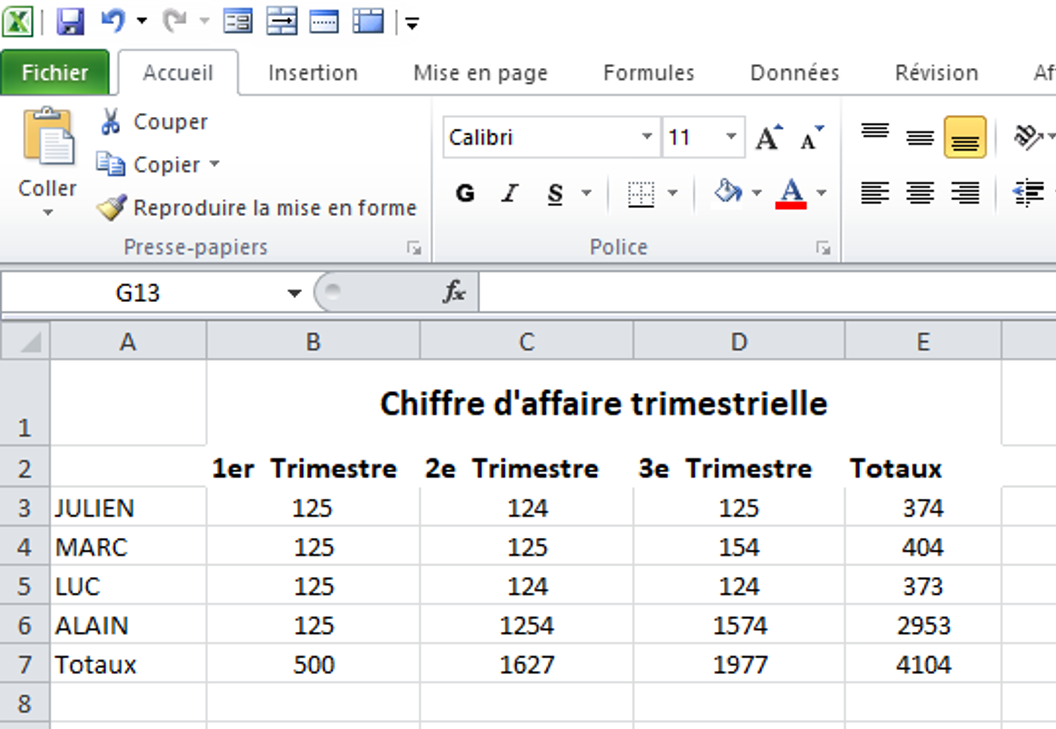
\includegraphics[scale=0.2,width=0.7 \linewidth]{img/ex03} 
	\captionof{figure}{Exercice \ref{ex3}} 
\end{figure} 

\begin{exercice}\label{ex1}
	Consignes :
 	\begin{enumerate}
 				
 	\item  Copier le Tableau de l'exercice \ref{ex03} dans une nouvelle feuille .  				
 	\item  Mettre la mise en forme le tableau: bordures, Trames, style titre en gras, taille de police: titre=12, autre=11, police Calibri.				
 	\item  Saisir le titre et le centrer horizontalement et veriticalement.				
 	\item  Utiliser le format nombre: 3 chiffre apres la virgule ainsi le separateur de mille.				
 		
 	\end{enumerate}
\end{exercice}  
\begin{figure} [H]  
	\centering
	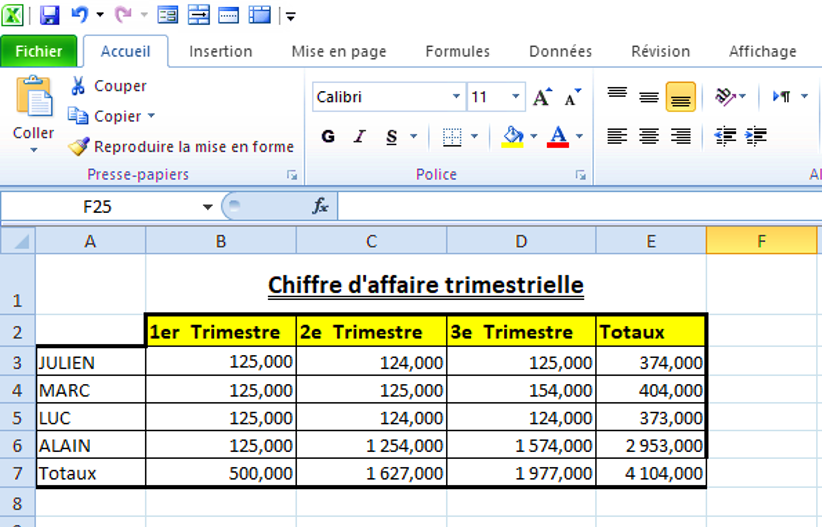
\includegraphics[scale=0.2,width=0.7 \linewidth]{img/ex01} 
	\captionof{figure}{Exercice \ref{ex1}} 
\end{figure}
\begin{exercice}\label{ex2}
	Consignes :
	\begin{enumerate}
		
		\item  Copier le Tableau de l'exercice \ref{ex1} dans une nouvelle feuille.  				
		\item  Mettre la mise en forme le tableau: bordures, Trames, style titre en gras, taille de police: titre=12, autre=11, police Calibri.				
		\item  Saisir le titre et le centrer horizontalement et veriticalement.				
		\item  Utiliser le format nombre: 3 chiffre apres la virgule ainsi le separateur de mille.
	\end{enumerate}	
\end{exercice}
\begin{figure}[H]
	\centering
	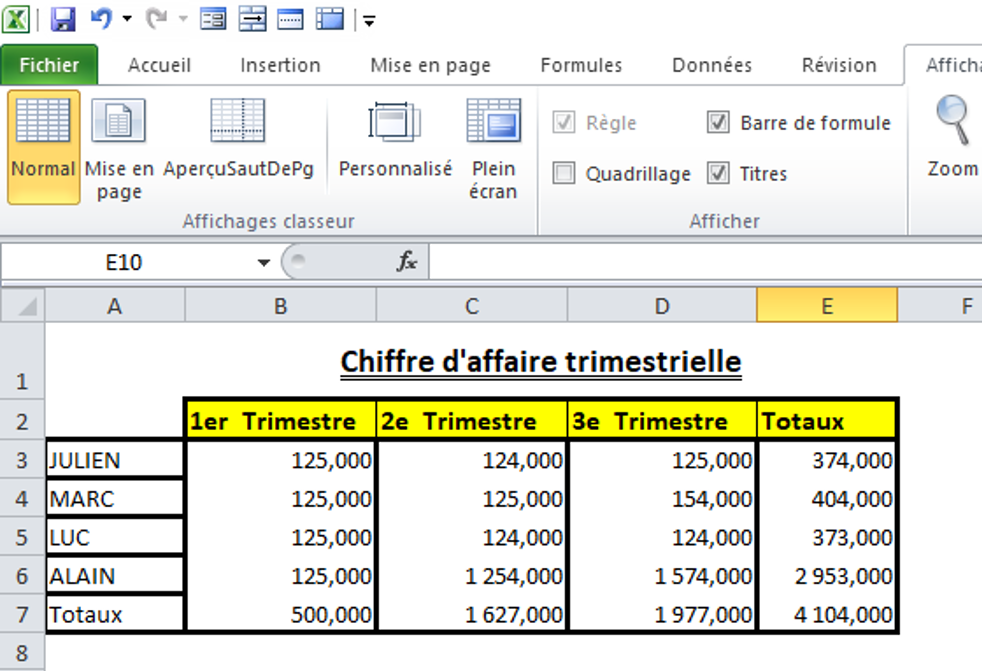
\includegraphics[scale=0.2,width=0.7 \linewidth]{img/ex02} 
	\captionof{figure}{Exercice \ref{ex2}} 
\end{figure}

 